\begin{figure}[H]
\centering
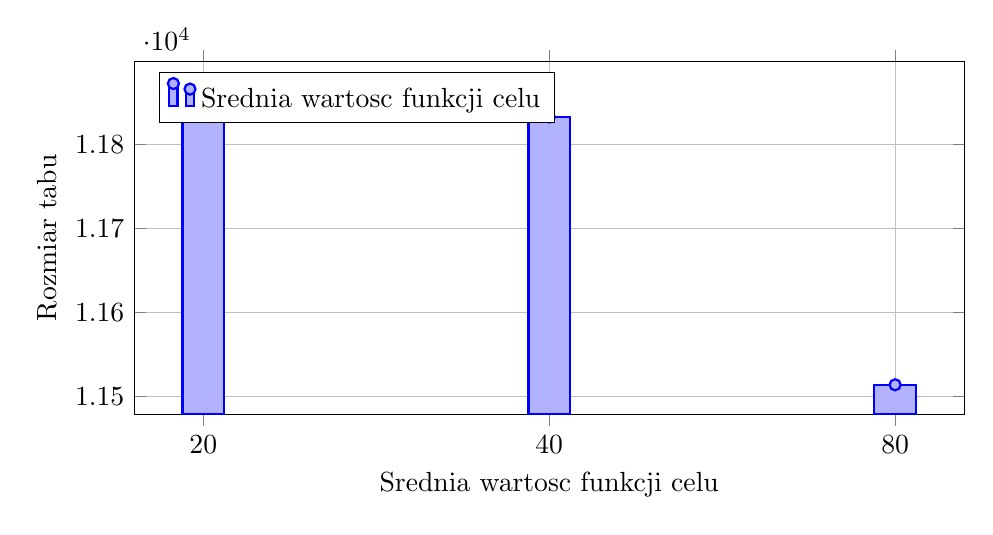
\begin{tikzpicture}
\begin{axis}[
xlabel = {Srednia wartosc funkcji celu},
ylabel = {Rozmiar tabu},
legend pos = north west,
grid = both,
width=1\linewidth,
height=0.5\linewidth,
ybar,
bar width=15pt,
symbolic x coords={20,40,80,},
xtick=data
]
\addplot + [mark = *, thick] coordinates
    {
(20,11864.208333333334)(40,11832.958333333334)(80,11514.041666666666)};
\addlegendentry
{Srednia wartosc funkcji celu}
\end{axis}
\end{tikzpicture}
\caption
{Srednia wartosc funkcji celu w zaleznosci od rozmiaru tabu dla wszystkich instancji}
\label{fig:mean_goals_per_tabu_size_all_instances}
\end{figure}
